\begin{framecard}
	{\color{colorbg}
	\bfseries

	\hugetext{Extensive form games\\\& their translation}}
\end{framecard}

\begin{frame}{Extensive form}
	\vspace{-3ex}
	\begin{center}
		\includegraphics[clip, page=12, trim=0cm 17cm 24cm 0cm, width=.65\textwidth]{figures/drawings.pdf}
	\end{center}

	\vfill
	\onslide<2->{
		\begin{definition}
			A \textbf{\textcolor{colornote}{(perfect information)} extensive-form tree} is a term of
			\begin{align*}
				\mbox{data} \;\PETree = \Leaf \;\; {\colar R}^{\colag P}\quad|\quad \Node \;\; \colag P \;\; \colar{(n : \N^+)}\;\; \colar{([n] \to  \PETree)}
			\end{align*}
			where $\colag P$ = set of \textbf{players}, $\colar R$ = type of \textbf{rewards} (usually $\R$).
		\end{definition}
	}
\end{frame}

\begin{frame}{Extensive form: strategies}
	%\textbf{\textcolor{coloragents}{Strategies}} can be inductively defined...
	\vspace{-3ex}
	\begin{center}
		\includegraphics[clip, page=13, trim=0cm 17cm 27cm 0cm, width=.5\textwidth]{figures/drawings.pdf}
	\end{center}
	\begin{definition}
		\vspace{-3ex}
		\begin{align*}
			& \colag{\strategies_\PET} : \PETree \to P \to \mathsf{Set} \\
			& \colag{\strategies_\PET} \; (\Leaf \; \colar v)\; \colag p = \colag\One \\
			& \colag{\strategies_\PET} \; (\Node \; \colag q \; \colar n \; f)\; \colag p\\
			& \qquad = (\mathsf{if}\ \colag{p \equiv q}\ \mathsf{then}\ \colag{[n]}\ \mathsf{else}\ \colag\One) \times (\Pi\,{\colar{m \in [n]}})\; \colag{\strategies_\PET}\; (f\; \colar{m)}\; \colag p\\
			% &\\
			% & \profiles_\PET : \PETree \to \mathsf{Set}\\
			% & \profiles_\PET\; T = (\Pi\,p \in P)\ \strategies_\PET\; T\; p
		\end{align*}
	\end{definition}
\end{frame}

\begin{frame}{Extensive form: moves}
	\begin{minipage}{\textwidth}
		\hspace{-5ex}
		\begin{minipage}{.51\textwidth}
			\begin{center}
				\includegraphics[clip, page=14, trim=1cm 17cm 26.2cm 0cm, width=\textwidth]{figures/drawings.pdf}
			\end{center}
			\begin{definition}
				\vspace{-3ex}
				\begin{align*}
					& \colar{\paths_\PET} : \PETree \to \mathsf{Set} \\
					& \colar{\paths_\PET} \; (\Leaf \; \colar v) = \colar \One \\
					& \colar{\paths_\PET} \; (\Node \; \colag p \; \colar n \; f) =\\ &\quad (\Sigma\,\colar{m \in [n]}) \; \colar{\paths_\PET}\; (f\; \colar m)
				\end{align*}
			\end{definition}
		\end{minipage}
		\hspace{3ex}
		\begin{minipage}{.5\textwidth}
			\begin{center}
				\includegraphics[clip, page=15, trim=1cm 17cm 26.2cm 0cm, width=\textwidth]{figures/drawings.pdf}
			\end{center}
			\begin{definition}
				\vspace{-3ex}
				\begin{align*}
					& \colar{\payoff_\PET} : (T : \PETree) \to (\paths_\PET\;T) \to \colar{R^P}\\
					& \colar{\payoff_\PET} \; (\Leaf \; \colar v) \; \colar\unit = \colar v\\
					& \colar{\payoff_\PET} \; (\Node \; \colag p \; \colar n \; f) \; \colar{(m, \pi)}\\
					&\quad = \colar{\payoff_\PET}\; (f\; \colar m) \; \colar \pi
				\end{align*}
			\end{definition}
		\end{minipage}
	\end{minipage}
\end{frame}

% \begin{frame}{Extensive form: payoff function}
% \end{frame}

% \begin{frame}{Extensive form}
% 	A game is presented as a (rooted) tree, which should reflect the possible unfoldings of the game.
% 	Each node is labelled with a \emph{player}. Branches represent possible \emph{moves} and \emph{payoff vectors} await at the leaves.

% 	Two kinds:
% 	\begin{enumerate}
% 		\item Perfect information: any player always knows exactly the state of the game (path from root to their nodes)
% 		\item Imperfect information: otherwise
% 	\end{enumerate}

% 	{\color{colornote}As customary in classical game theory, all players $\argmax$ their payoff.}
% \end{frame}

% \begin{frame}

% \end{frame}

\begin{frame}{Translation}
	Finally, we can translate any $\PETree$ to an open game with agency:

	% \begin{align*}
	% 	&\colar{\PETtoArena} : (T : \PETree) \longto \Lens_{\colag{(\Pi_p \strategies\, T\, p, R^P)}}\colar{(1,R^P)(\paths\; T, R^P)}\\
	% 	&\PETtoArena (\Leaf\; \colar v) = {\includegraphics[clip, page=18, trim=18cm 22cm 19cm 3.5cm, width=.1\textwidth]{figures/drawings.pdf}}\\
	% 	&\PETtoArena (\Node \; \colag p \; \colar n \; f) = {\includegraphics[clip, page=18, trim=18cm 7cm 1cm 10cm, width=.65\textwidth]{figures/drawings.pdf}}
	% \end{align*}
	\vfill
	\begin{minipage}{\textwidth}
		\hspace{-9ex}
		\begin{minipage}{1.15\textwidth}
			\begin{center}
				\includegraphics[clip, page=18, trim=0cm 11.5cm 5cm 0cm, width=\textwidth]{figures/drawings.pdf}
			\end{center}
		\end{minipage}
	\end{minipage}

	\vfill
	and we equip this arena with $\colag{\boxtimes_{p \in P} \argmax (- \cmp \pi_p)}$.
\end{frame}

\begin{frame}{Imperfect information}
	Sometimes players can't access the whole state of the game (i.e. history of play)

	\vfill
	\begin{center}
		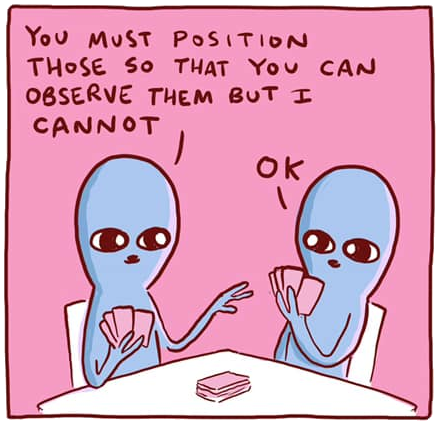
\includegraphics[width=.65\textwidth]{figures/imperfect-information.png}
	\end{center}
\end{frame}

\begin{frame}{Imperfect information}
	Access to information (or better, lack thereof) is represented by sets of 'indistinguishable states' called \textcolor{coloragents}{\textbf{information sets}}:

	\begin{center}
		{\includegraphics[clip, page=16, trim=0cm 16cm 26.2cm 0cm, width=.7\textwidth]{figures/drawings.pdf}}
	\end{center}


	\vfill
	\textbf{Limit case}: all information sets are singletons $\equiv$ perfect information.
\end{frame}

\begin{frame}{Imperfect information}
	\textcolor{coloragents}{Strategies} need to respect information sets: players can't distinguish between states in the same set:

	\begin{center}
		\includegraphics[clip, page=17, trim=0cm 13.5cm 11cm 0cm, width=.9\textwidth]{figures/drawings.pdf}
	\end{center}

	\textcolor{colornote}{It gets a bit more complicated with mixed strategies.}
\end{frame}


\begin{frame}{Adding imperfect information}
	\begin{definition}
		An \textbf{imperfect information extensive-form tree} is a term of
		\begin{align*}
			\mbox{data} \;\; \IETree = \Leaf \;\; {\colar R}^{\colag P} \ |\  \Node \;\; \colag{(i:I)} \;\; \colar{([n\; i] \to  \IETree)}
		\end{align*}
		where
		\begin{enumerate}
			\item $\colag{I : \Set}$ is a set of \textbf{information labels},
			\item  $\colar{n : I \to \N^+}$ assigns moves to nodes of the same information set and
			\item there is a \textcolor{colornote}{(surjective)} map $\colag{\belongs : I \to P}$.
		\end{enumerate}
	\end{definition}
\end{frame}


\begin{frame}{Translation}
	\textbf{Idea}: information sets are instances of 'tying':
	\begin{enumerate}
		\item Forget about information sets and recover a perfect information game:
		\begin{align*}
			& \IETtoPET : \IETree \to \PETree\\
			& \IETtoPET\; (\Leaf\; \colar v) = \Leaf\; \colar v\\
			& \IETtoPET\; (\Node\; \colag i\; f) = \Node\; (\colag{\belongs\;i})\; (\colar{n\; i})\; (\lambda \colar{m} \,.\, \IETtoPET\; (f\; \colar m))
		\end{align*}
		\item Translate it using $\PETtoArena$.
		\item Reparametrise along $\colag\clone$ which ties strategies in the same information sets.
	\end{enumerate}
	\begin{align*}
		\colag{\IETtoArena}(T) = \colag{\clone^*} (\colar{\PETtoArena}\; (\IETtoPET\; T))
	\end{align*}
\end{frame}

\begin{frame}{Example: Prisoner's Dilemma}
	\vspace{-7ex}
	\begin{flushright}
		\hspace{5ex}
		\includegraphics[clip, page=20, trim=0cm 18.5cm 25cm .5cm, width=.4\textwidth]{figures/drawings.pdf}
	\end{flushright}
	\begin{center}
		\includegraphics[clip, page=21, trim=0cm 0cm 0cm 0cm, width=.9\textwidth]{figures/drawings.pdf}
	\end{center}
\end{frame}

\begin{frame}{Example: Prisoner's Dilemma}
	\begin{center}
		\includegraphics[clip, page=22, trim=0cm 13cm 15cm 0cm, width=.7\textwidth]{figures/drawings.pdf}
	\end{center}
\end{frame}
